\documentclass{beamer}
% colors
\usepackage{color}    
\usepackage[table]{xcolor}
\usepackage{themecolors}

\usetheme{Boadilla}

\definecolor{UBCblue}{rgb}{0.04706, 0.13725, 0.26667} % UBC Blue (primary)

\usecolortheme[named=green2]{structure}

\usepackage[utf8]{inputenc}
\usepackage{amsmath, amssymb}
\usepackage[T1]{fontenc}

% tikz stuff
\usepackage{tikz} 
\usetikzlibrary{positioning, shapes.multipart, arrows, arrows.meta, shadows, backgrounds, fit}

% isabelle blocks
\usepackage{listings}
\lstdefinelanguage{isabelle}{%
    keywords=[1]{type_synonym,datatype,fun,abbreviation,definition,proof,lemma,theorem,session,sessions,theories,text,section},
    keywordstyle=[1]\bfseries\color{isabelleouterblue},
    keywords=[2]{where,assumes,shows,and},
    keywordstyle=[2]\bfseries\color{isabelleoutergreen},
    keywords=[3]{if,then,else,case,of,SOME,let,in,O},
    keywordstyle=[3]\color{isabelleinnerblue},
    keywords=[4]{apply, by, done},
    keywordstyle=[4]\color{isabelleoutersalmon},
    morestring=[b]",
    morecomment=[n]{(*}{*)},
    % morecomment=[n]{\guilsingleft}{\guilsingright},
    stringstyle=\color{isabellequote},
    showstringspaces=false,
}
\lstdefinelanguage{file}{
}
\lstset{%
  language=isabelle,
  escapeinside={&}{&},
  columns=fixed,
  extendedchars,
  basewidth={0.5em,0.45em},
  basicstyle=\ttfamily,
  mathescape,
}

\title{Stacking Correspondence}
\subtitle{Formal Verification of a Network Stack}
\author{Daniel Neshyba-Rowe}
\institute{Lewis \& Clark}
\date{April 17, 2025}
\begin{document}

\begin{frame}<1>[label=title]
\titlepage
\end{frame}

% \begin{frame}
% \frametitle{Outline}
% \tableofcontents
% \end{frame}

\section{Introduction}

\subsection{The Network Stack}
\begin{frame}{The Network Stack}
    

    \begin{itemize}
        \item<1-> ``the network stack is an implementation of a computer networking protocol suite or protocol family'' (wikipedia)
        \begin{itemize}
            \item<2-> not a very helpful description
            \item<2-> engineering solution to a difficult problem \\(routing, reliability, resolution)
        \end{itemize}
        
    \end{itemize}
    

    \onslide<1,2>{
    \begin{figure}
        \centering
        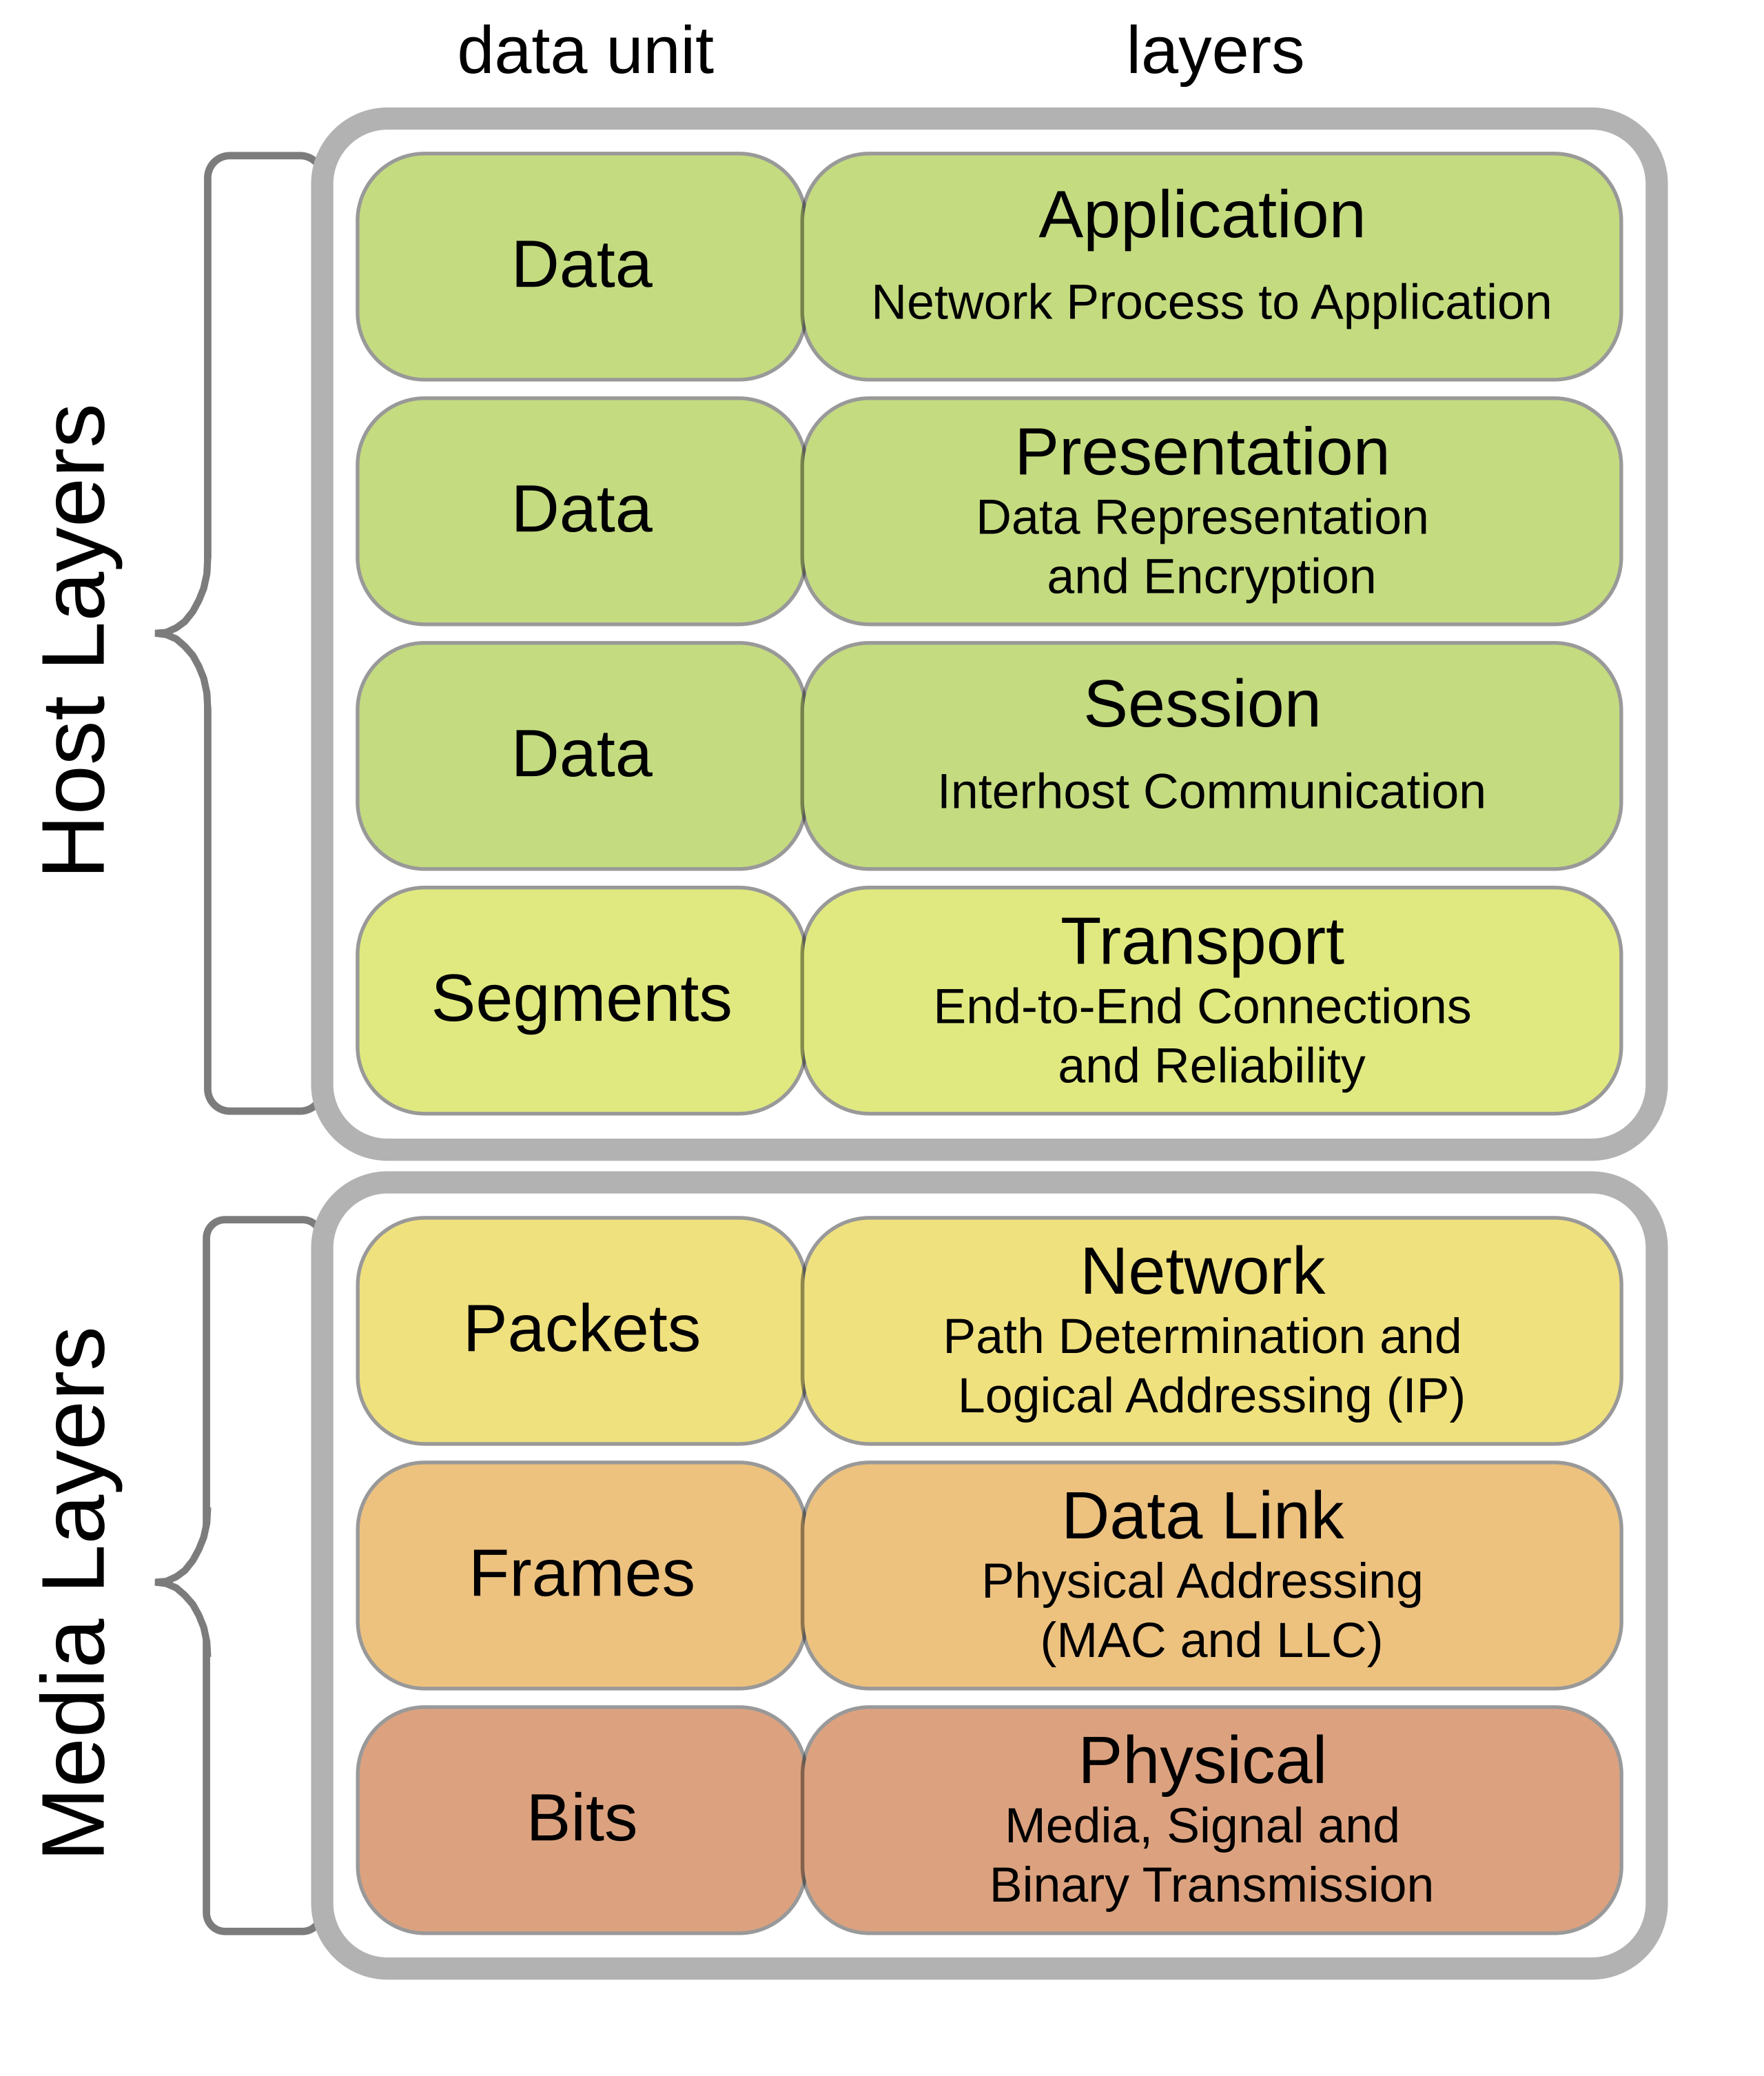
\includegraphics[width=0.35\linewidth]{../thesis_presentation/figs/wikipedia_OSI_Model_v1.svg.png}
        \caption{The OSI model, taken from Wikipedia}
        \label{fig:enter-label}
    \end{figure}
    }
\end{frame}

\begin{frame}{The Network Stack---Post Office analogy}
\begin{columns}
    \column{0.5\textwidth}
    \begin{figure}
        \centering
        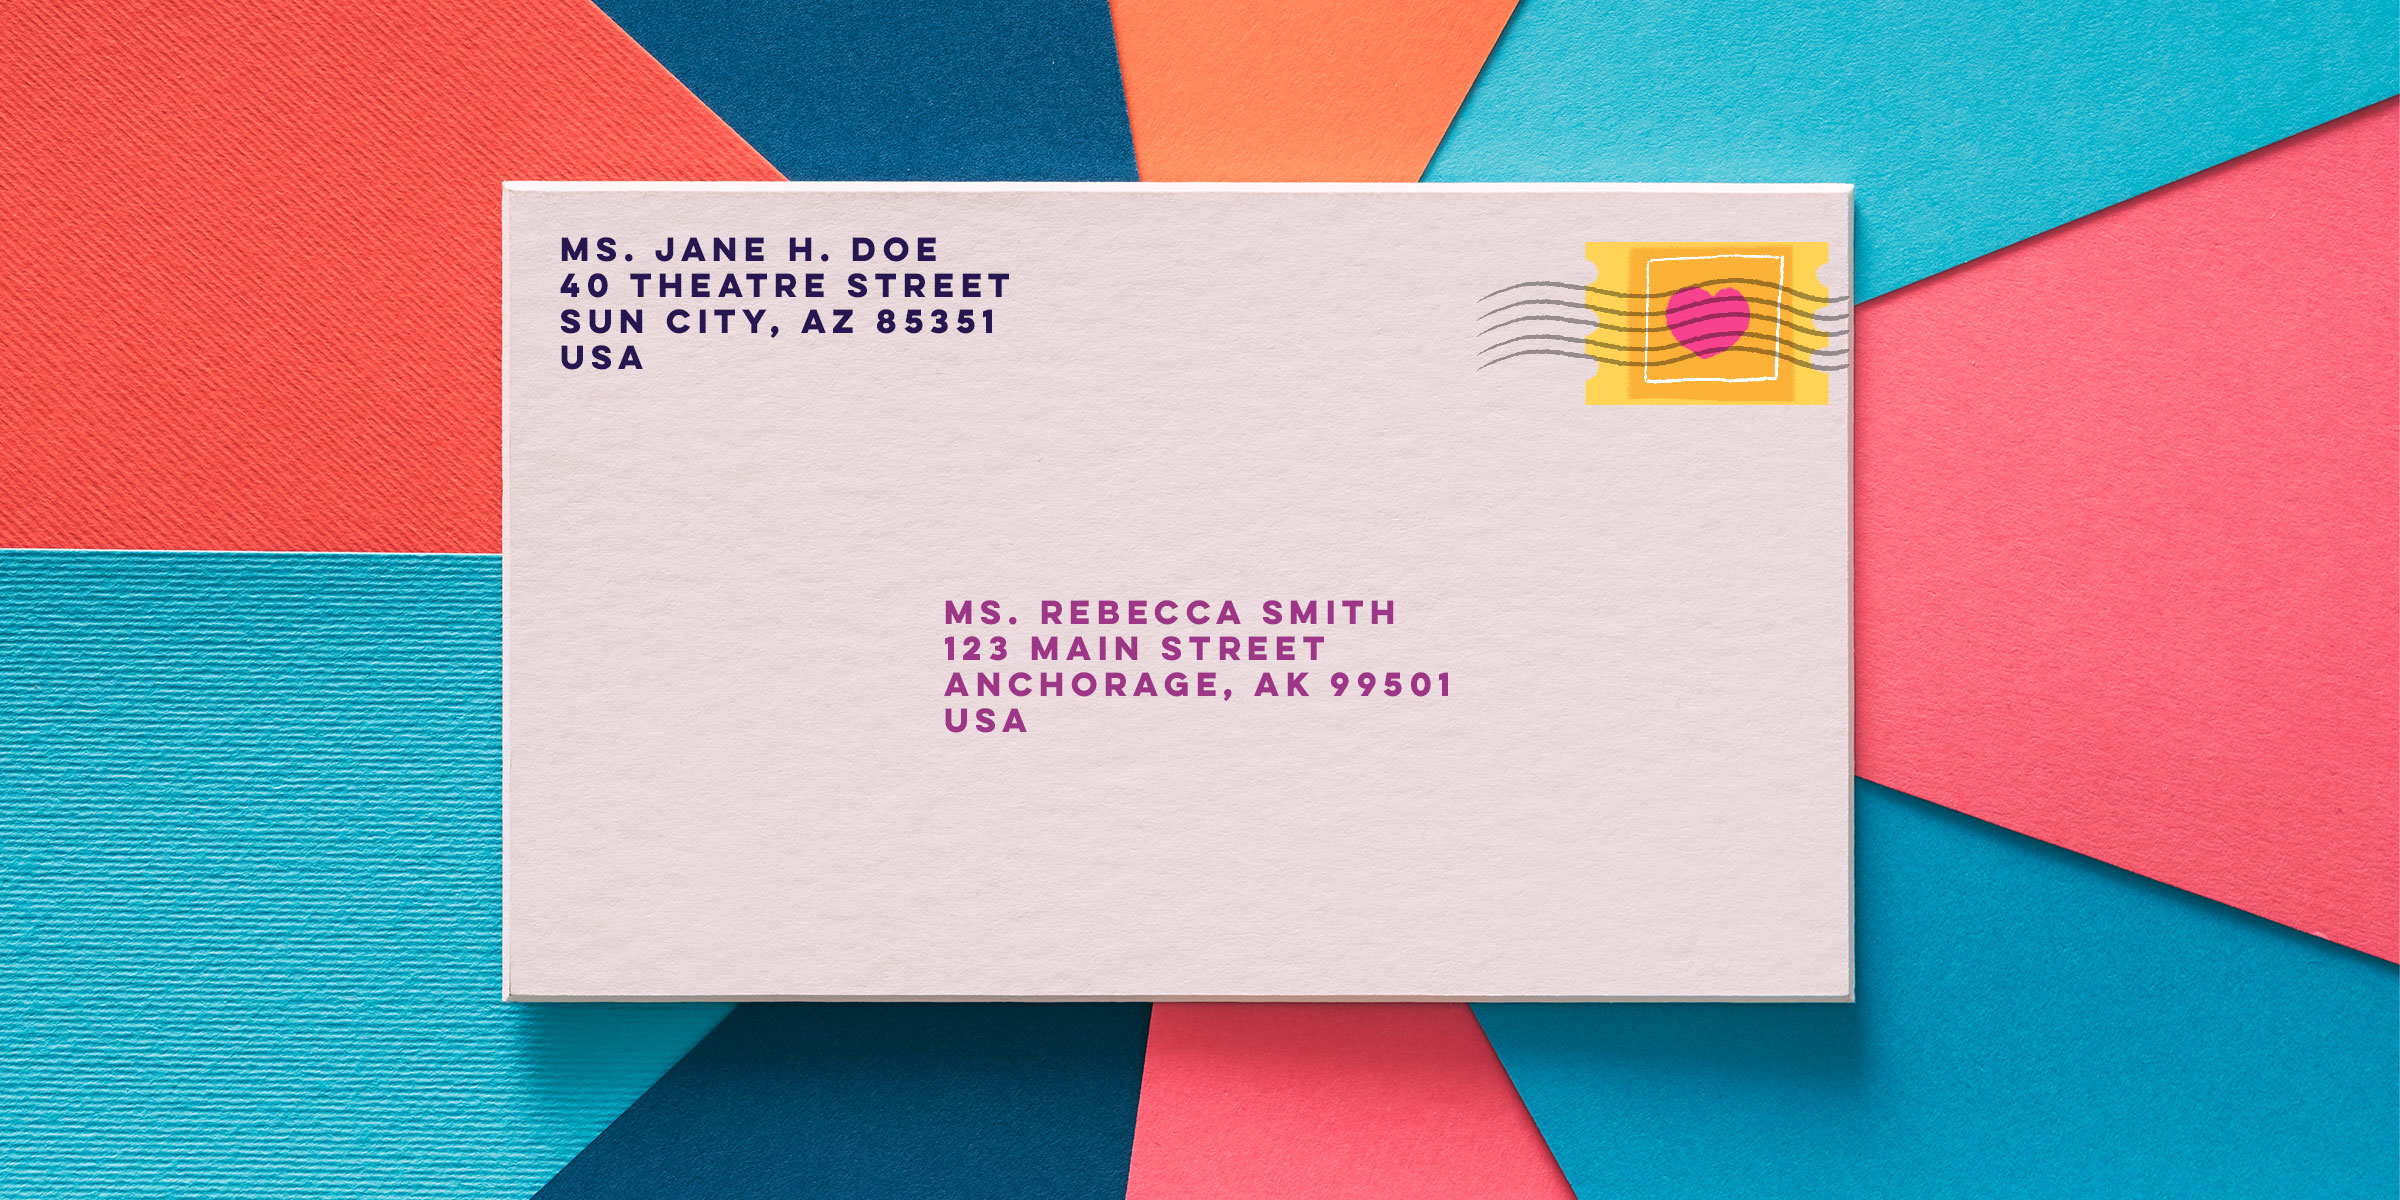
\includegraphics[height=0.5\linewidth]{../thesis_presentation/figs/envelope.jpg}
    \end{figure}
    
    \begin{figure}
        \centering
        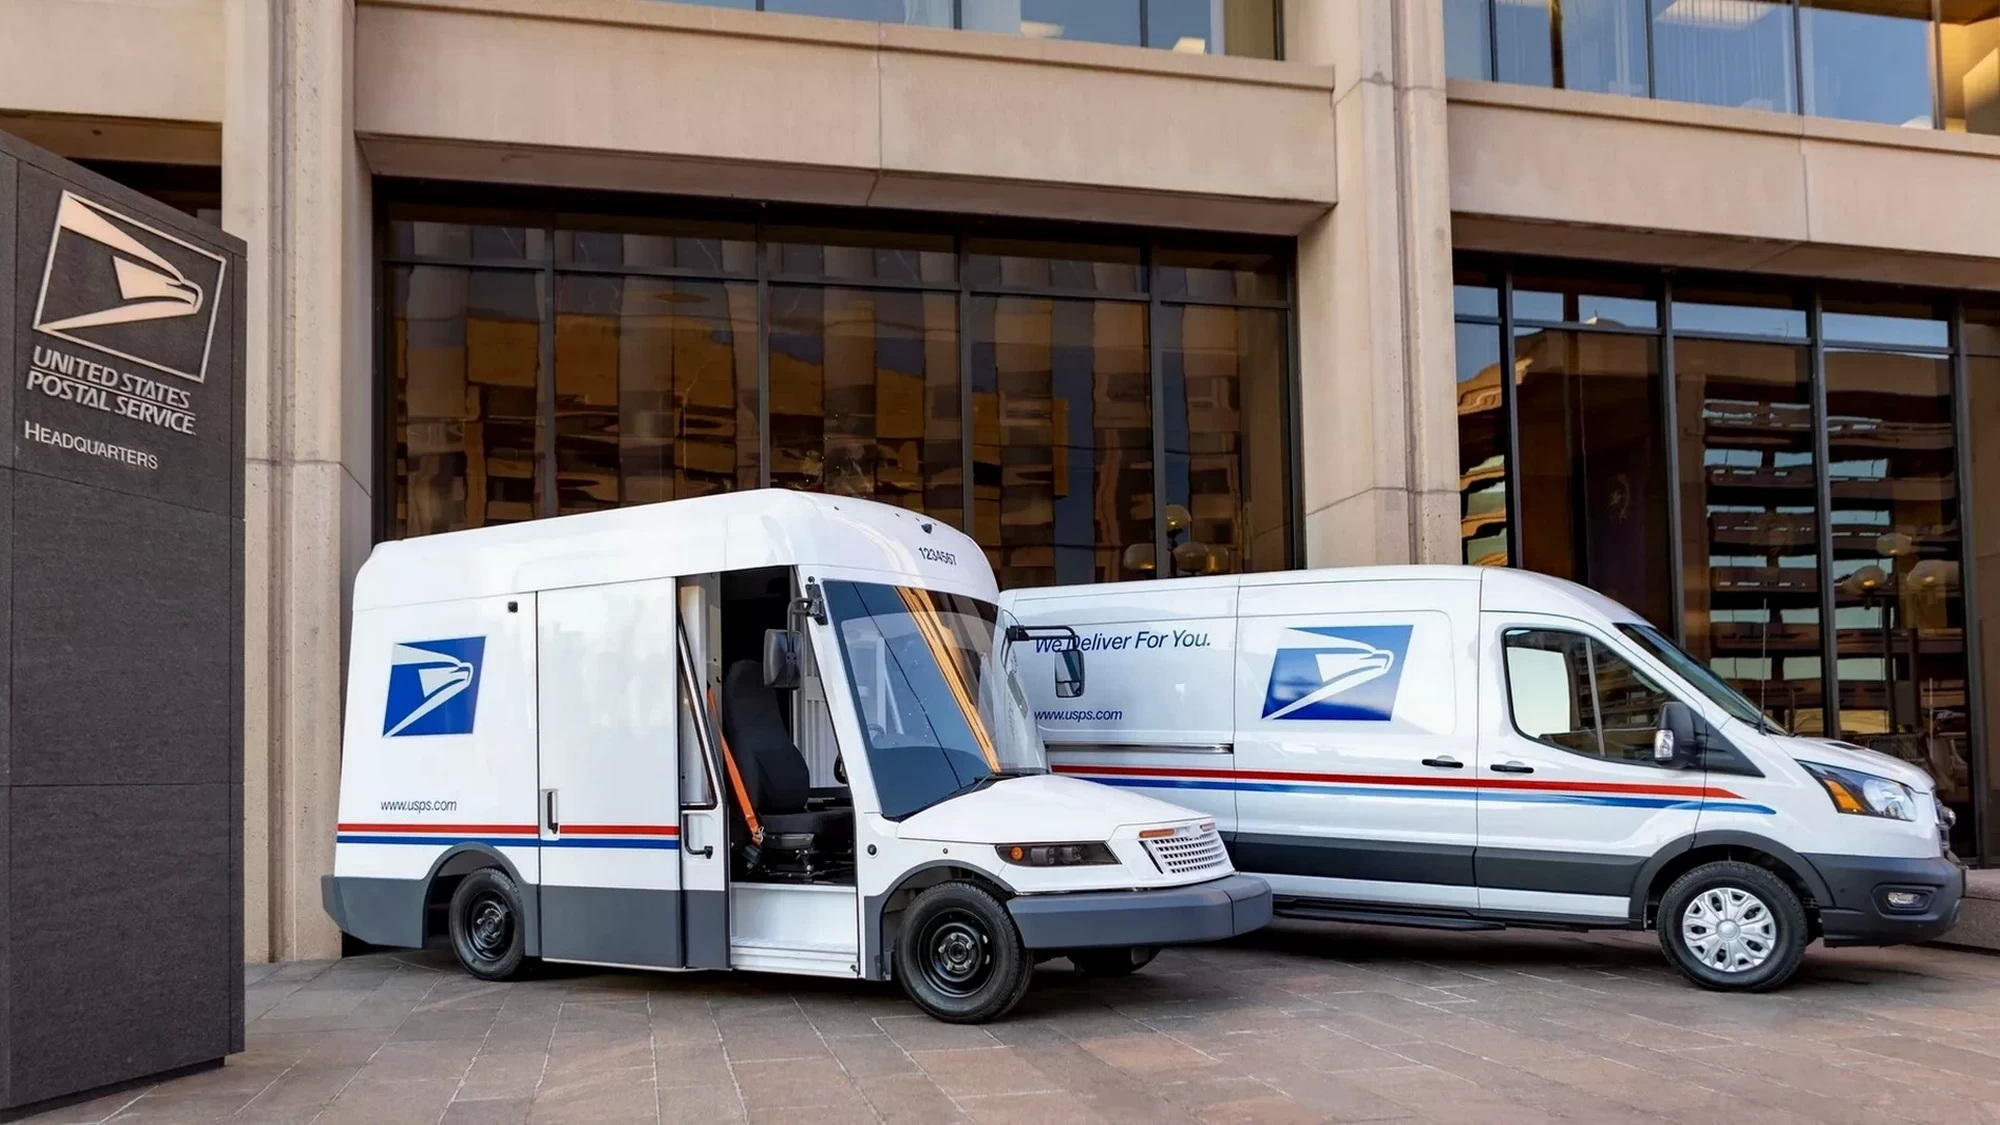
\includegraphics[height=0.5\linewidth]{../thesis_presentation/figs/post_truck.jpg}
    \end{figure}
    
    \column{0.5\textwidth}
    
    \begin{figure}
        \centering
        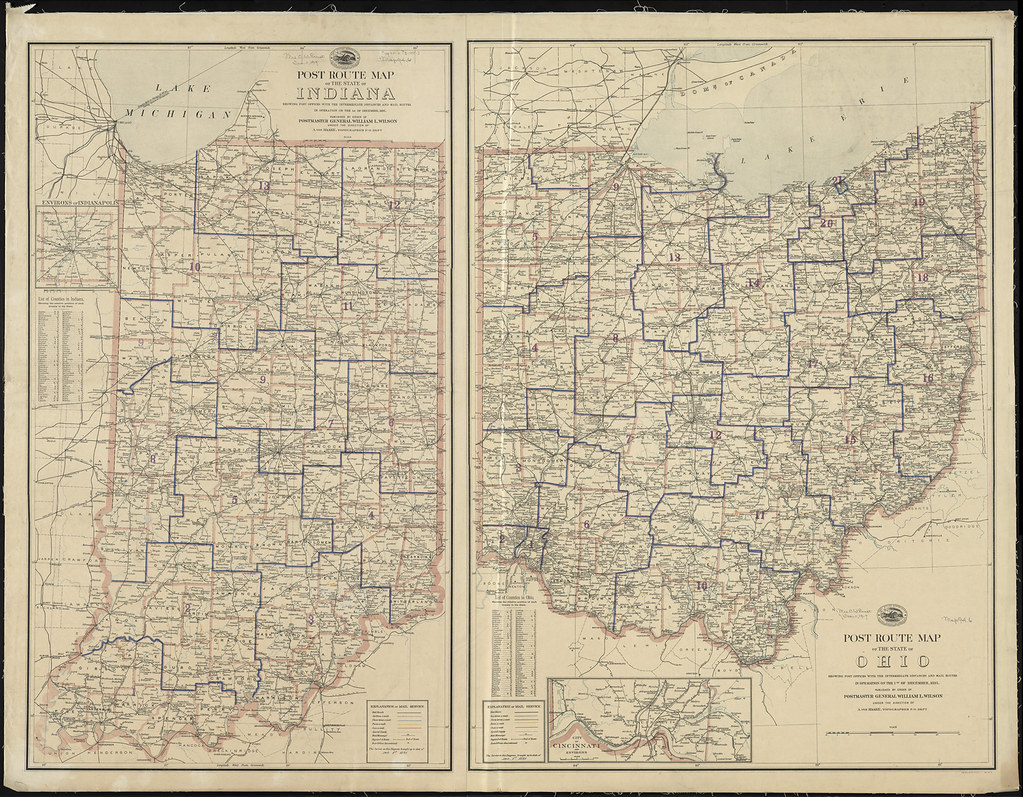
\includegraphics[height=0.5\linewidth]{../thesis_presentation/figs/post_routes.jpg}
    \end{figure}
    
    \begin{figure}
        \centering
        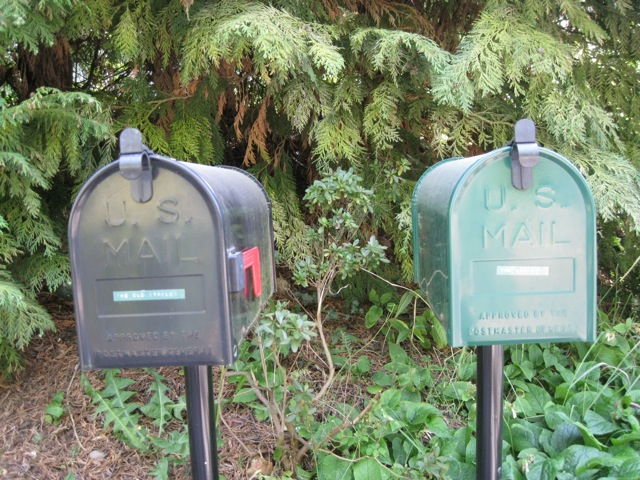
\includegraphics[height=0.5\linewidth]{../thesis_presentation/figs/post_neighborhood.jpg}
    \end{figure}
    
\end{columns}
\end{frame}

\begin{frame}<1,2>[label=verification_rough]
\frametitle<1,3>{Verification}
\frametitle<2>{Verification \textit{(foreshadowing)}}

Verification is proving ``it has no bugs.''
But what does that look like?

    \begin{columns}[t]
        \column{0.5\textwidth}<1->
        \begin{itemize}
            \item imagine an ideal post office
        \end{itemize}
        \column{0.5\textwidth}<2->
        \begin{itemize}
            \item created an \alert<2>{\it abstract specification} of UDP\_wrap
        \end{itemize}
    \end{columns}
    
    \begin{columns}[t]
        \column{0.5\textwidth}<1->
        \begin{itemize}
            \item show that the ideal post office works great
            \begin{itemize}
                \item letters I send to you, you receive as written
            \end{itemize}
        \end{itemize}
        \column{0.5\textwidth}<2->
        \begin{itemize}
            \item wrote formal statements in isabelle saying various \alert<2>{\it invariants} hold in the abstract specification
        \end{itemize}
    \end{columns}

    \begin{columns}[t]
        \column{0.5\textwidth}<1->
        \begin{itemize}
            \item look at a real post office
            \vspace{\baselineskip}\\
            \item show that the real post office works the same as the theoretical one
        \end{itemize}
        
        \column{0.5\textwidth}<2->
        \begin{itemize}
            \item created a \alert<2>{\it design specification} of UDP\_wrap
            \item wrote formal statements saying the design specification \alert<2>{\it refines/corresponds to} the abstract specification
        \end{itemize}
    
    \end{columns}
    
\end{frame}

\begin{frame}<1,2>[label=ver_dif_tests]{Formal Verification is different from tests}

    ``Testing shows the presence, not the absence of bugs'' - Dijkstra
    \vspace{20pt}
    
    In formal verification, we need rigorous mathematical proofs.
    
    Furthermore, these proofs should be verified
    by a \alert<2,3,4>{\it proof engine}.
    \vspace{20pt}
    
    One challenge with \alert<4>{system software} (e.g. linux kernel, drivers) is that things
    frequently have a low chance of failing, but could still fail (e.g. two processes trying to access
    the same data at the same time---unlikely, but
    if handled poorly disastrous).
\end{frame}

\begin{frame}{Proof engines make proofs more rigorous}
    Infamously, people make misatkes.
    This is a big problem when formality is required.

    % TODO: split up into own slide? Ignore?
    Some examples of human error in proofs:
    \begin{itemize}
        \item fifth postulate
        \item all horses are the same color
    \end{itemize}

    What's the solution?
    Use software to automate checking proofs (a proof engine).

\end{frame}

\begin{frame}[fragile]{Isabelle --- the proof engine we use}
    Isabelle is one such proof engine.
    Isabelle is itself verified correct, and provides tools to prove mathematical statements.
    \begin{lstlisting}
lemma "2 + 2 = 4" by simp
    \end{lstlisting}
\end{frame}

\againframe<3,4>{ver_dif_tests}

\againframe<2>{title}



\subsection{Goals}
% \begin{frame}
%     \frametitle{Alain's big-picture for Dependable Computing}
%     \begin{itemize}
%         \item Explore formal code
%             \begin{itemize}
%                 \item lots of existing high-level verification
%                 \item seL4 first verified microkernel
%                 \item how far up can we push it?
%             \end{itemize}
%         \item Build a significant program correctly
%             \begin{itemize}
%                 \item embedded system
%                 \item IPv6 networked fish tank thermometer
%                 \item network communication definitely not trivial
%             \end{itemize}
%     \end{itemize}
% \end{frame}

\begin{frame}
    \frametitle{Goals for my part of the project}
        \begin{itemize}
            \item eventually, build a fully functional networked fish tank thermometer, and formally verify it.
            \item start on some of the simpler parts of proof, for a small part of the network stack
            \item gain insight into how our proofs should work
        \end{itemize}
\end{frame}

\begin{frame}
    \frametitle{Our network stack for a fish tank thermometer}
\begin{figure}[htpb]
    \centering
    \scalebox{0.65}{
    \begin{tikzpicture}[node distance=4cm]
        % styles
        \tikzstyle{cell} = [rectangle, minimum width=4.6cm, minimum height=1cm, text centered, draw=black]
        \tikzstyle{arrow} = [line width=2pt,->,>=latex,draw=gray]
        \tikzstyle{box} = [draw, rectangle, align=center, minimum width=11cm, inner sep=3ex]

        % wrap
        \node (app_wrap) [cell, fill=application!80] {Application on Computer A};
        \node (udp_wrap) [cell, fill=udp!80, below=35pt of app_wrap] {UDP wrap};
        \node at (udp_wrap) [rectangle, minimum width=4.6cm, minimum height=1cm, draw=black, line width=1mm] {};
        \node (ip_wrap) [cell, fill=ip!80, below=35pt of udp_wrap] {IP wrap};
        \node (ethernet_wrap) [cell, fill=ethernet!80, below=35pt of ip_wrap] {Ethernet wrap};
        \node (hardware_wrap) [cell, fill=hardware!80, below=35pt of ethernet_wrap] {Hardware};

        % unwrap
        \node (app_unwrap) [cell, fill=application!80, right=14pt of app_wrap] {Application on Computer B};
        \node (udp_unwrap) [cell, fill=udp!80, below=35pt of app_unwrap] {UDP unwrap};
        \node (ip_unwrap) [cell, fill=ip!80, below=35pt of udp_unwrap] {IP unwrap};
        \node (ethernet_unwrap) [cell, fill=ethernet!80, below=35pt of ip_unwrap] {Ethernet unwrap};
        \node (hardware_unwrap) [cell, fill=hardware!80, below=35pt of ethernet_unwrap] {Hardware};

        % layers
        \node[box, label={left:\rotatebox{90}{Higher-level}}, fit = (app_wrap) (app_unwrap)] (1) {};
        \node[box, label={left:\rotatebox{90}{Transport}}, fit = (udp_wrap) (udp_unwrap)] (1) {};
        \node[box, label={left:\rotatebox{90}{Network}}, fit = (ip_wrap) (ip_unwrap)] (1) {};
        \node[box, label={left:\rotatebox{90}{Data Link}}, fit = (ethernet_wrap) (ethernet_unwrap)] (1) {};
        \node[box, label={left:\rotatebox{90}{Physical}}, fit = (hardware_wrap) (hardware_unwrap)] (1) {};

        % flow of information
        \draw [arrow] (app_wrap) -- (udp_wrap);
        \draw [arrow] (udp_wrap) -- (ip_wrap);
        \draw [arrow] (ip_wrap) -- (ethernet_wrap);
        \draw [arrow] (ethernet_wrap) -- (hardware_wrap);
        \draw [arrow] (hardware_wrap) -- (hardware_unwrap);
        \draw [arrow] (hardware_unwrap) -- (ethernet_unwrap);
        \draw [arrow] (ethernet_unwrap) -- (ip_unwrap);
        \draw [arrow] (ip_unwrap) -- (udp_unwrap);
        \draw [arrow] (udp_unwrap) -- (app_unwrap);
    \end{tikzpicture}}
    % \label{fig:network-stack}
\end{figure}
UDP = ``User Datagram Protocol''
\end{frame}

\begin{frame}<1>[fragile, label=rfc]{What does UDP\_wrap look like?}
Excerpt from RFC 768 (RFC=Request For Comment)

\begin{lstlisting}[language=file]
                  0      7 8     15 16    23 24    31
                 +--------+--------+--------+--------+
                 |     Source      |   Destination   |
                 |      Port       |      Port       |
                 +--------+--------+--------+--------+
                 |                 |                 |
                 |     Length      |    Checksum     |
                 +--------+--------+--------+--------+
                 |
                 |          data octets ...
                 +---------------- ...

                      User Datagram Header Format
\end{lstlisting}
\end{frame}

\againframe<3>{verification_rough}

\begin{frame}{How the proofs look}
    \begin{figure}
        \centering
        \scalebox{0.5}{
        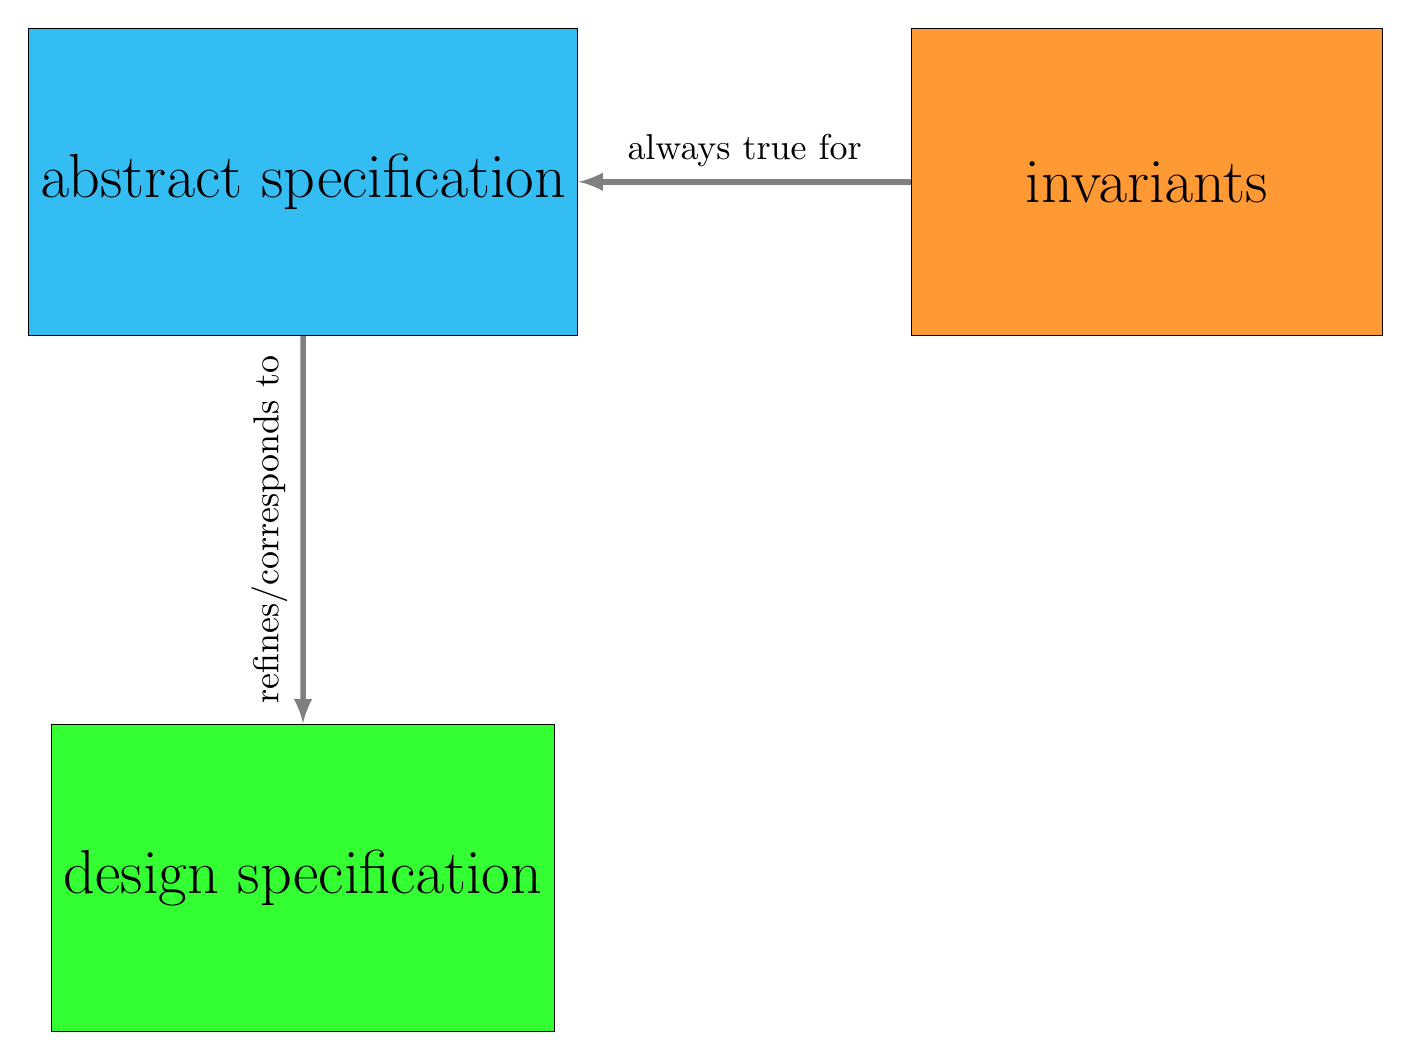
\begin{tikzpicture}[node distance=4cm, every node/.style={scale=1.3}]
            % styles
            \tikzstyle{cell} = [rectangle, minimum width=4.6cm, minimum height=3cm, text centered, draw=black]
            \tikzstyle{arrow} = [line width=2pt,->,>=latex,draw=gray]
            \tikzstyle{box} = [draw, rectangle, align=center, minimum width=11cm, inner sep=3ex]
    
            % wrap
            \node (abstract) [cell, fill=cyan!80] {\LARGE abstract specification};
            \node (invs) [cell, fill=orange!80, right=120pt of abstract] {\LARGE invariants};
            \node (design) [cell, fill=green!80, below=140pt of abstract] {\LARGE design specification};
            
            % \node [color=red] at (0, -150pt) {blocked access};
            % \node [color=green!200] at (-115pt, -180pt) {good access};
    
            % flow of information
            \draw [arrow] (abstract) -- (design) node[midway, left] {\rotatebox{90}{refines/corresponds to}};
            \draw [arrow] (invs) -- (abstract) node[midway, above] {always true for};
        \end{tikzpicture}}
    \end{figure}
\end{frame}


\begin{frame}[fragile]{Invariants}
    \begin{lstlisting}[language=isabelle]
lemma compose_to_id:
"VARS orig_msg wrapped_msg unwrapped_msg conn
&\colorbox{green}{\{well\_formed orig\_msg conn\}}&
&\colorbox{cyan}{wrapped\_msg := udp\_wrap orig\_msg conn;}&
&\colorbox{cyan}{unwrapped\_msg := udp\_unwrap wrapped\_msg}&
&\colorbox{blue}{\{orig\_msg = unwrapped\_msg\}}&"
    \end{lstlisting}

    \pause
    \vspace{20pt}
    This is a type of \textit{Hoare triple}, which are statements of the form
    \begin{lstlisting}[language=isabelle]
&\colorbox{green}{\{precondition\}}&
&\colorbox{cyan}{program that changes state}&
&\colorbox{blue}{\{postcondition\}}&
    \end{lstlisting}
\end{frame}


\begin{frame}[fragile]{Abstract specification types}
    \begin{lstlisting}[language=isabelle]
type_synonym message = "nat list"

type_synonym ip_addr = "nat"
type_synonym port = "nat"
type_synonym socket = "ip_addr $\times$ port"
type_synonym connection = "socket $\times$ socket"

    \end{lstlisting}
\end{frame}

\begin{frame}[fragile]{Design specification types}
    \begin{lstlisting}[language=isabelle]
type_synonym message_d = "byte list"

(* IPv6 addresses are 8 16-bit words *)
type_synonym ip_addr_d = "word16 $\times$ word16 $\times \cdots \times$ word16"
type_synonym port_d = "word16"
type_synonym socket_d = "ip_addr_d $\times$ port_d"
type_synonym connection_d = "socket_d $\times$ socket_d"
    \end{lstlisting}
\end{frame}

\begin{frame}[fragile]{Abstract specification}
    \begin{lstlisting}[language=isabelle]
fun udp_wrap :: "message $\Rightarrow$ connection $\Rightarrow$ message" where
  "udp_wrap msg conn = (let
                          src_sk = src conn;
                          dst_sk = dst conn;
                          src_ip_addr = ip_addr src_sk;
                          dst_ip_addr = ip_addr dst_sk;
                          src_port = port src_sk;
                          dst_port = port dst_sk;
                          len = length msg + udp_hdr_sz
                        in
                          [src_port, dst_port, len,
                           checksum16 [src_ip_addr,
                                       dst_ip_addr,
                                       0, udp_proto, len]
                          ]) @ msg"
    \end{lstlisting}
\end{frame}

\againframe<2>{rfc}


\begin{frame}[fragile]{Design specification}
    \begin{lstlisting}[language=isabelle]
fun udp_wrap_d :: "message_d $\Rightarrow$ connection_d $\Rightarrow$ message_d"
where "udp_wrap_d msg conn = (let
                            src_sk = src conn;
                            dst_sk = dst conn;
                            src_ip_addr = ip_addr src_sk;
                            dst_ip_addr = ip_addr dst_sk;
                            src_port = port src_sk;
                            dst_port = port dst_sk;
                            len = (of_nat
                        (length msg + udp_hdr_sz)::word16);
                            chksum = (0 :: word16)
                          in
                            (porttomsgd src_port @
                             porttomsgd dst_port @
                             w16tomsg len @
                             w16tomsg chksum
                            ) @ msg)"


    \end{lstlisting}
\end{frame}

\begin{frame}{Refinement / Correspondence}
In order to show the design specification refines/corresponds to the abstract specification,
we first need a sense of correspondence between two things
\begin{itemize}
    \item messages
    \item connections
\end{itemize}
\end{frame}

\begin{frame}[fragile]{Refinement / Correspondence -- messages}
    
    \begin{lstlisting}[language=isabelle]
fun relation_message :: "message $\Rightarrow$ message_d $\Rightarrow$ bool"
  where
    "relation_message [] [] = True" |
    "relation_message ms [] = False" |
    "relation_message [] ms' = False" |
    "relation_message (m#ms) (m'#ms') = (
            (m = unat m') $\land$ relation_message ms ms'
      )"


    \end{lstlisting}
\end{frame}

\begin{frame}[fragile]{Refinement / Correspondence -- connections}
    \begin{lstlisting}[language=isabelle]
fun ip_addr_d_to_nat :: "ip_addr_d $\Rightarrow$ nat" where
  "ip_addr_d_to_nat (a,b,c,d,e,f,g,h) = (unat a)*2^(16*7) +
                                        (unat b)*2^(16*6) +
                                        $\vdots$
                                        (unat h)*2^(16*0)"
definition relation_socket :: "socket $\Rightarrow$ socket_d $\Rightarrow$ bool"
  where "relation_socket sock sock_d $\equiv$ (
    (ip_addr_a sock = ip_addr_d_to_nat (ip_addr_d sock_d)) $\land$
    (port_a sock = unat (port_d sock_d))
        )"
definition relation_connection :: "connection $\Rightarrow$ connection_d
                                   $\Rightarrow$ bool"
  where "relation_connection con con_d $\equiv$ (
              relation_socket (src_a con) (src_d con_d) $\land$
              relation_socket (dst_a con) (dst_d con_d)
        )"
    \end{lstlisting}
\end{frame}

\begin{frame}[fragile]{Formal statement of refinement/correspondence}

``Every possible result of the design specification is an allowed result of the abstract specification.''

    \begin{lstlisting}[language=isabelle]
theorem "relation_message msg msg_d $\Longrightarrow$
         relation_connection conn conn_d $\Longrightarrow$
         relation_message (udp_wrap msg conn)
                          (udp_wrap_d msg_d conn_d)"
    \end{lstlisting}
\end{frame}

\begin{frame}{Conclusions}
    \begin{itemize}
        \item What does formal verification look like in our case?
        \begin{itemize}
            \item abstract specification
            \item show invariants hold for abstract specification
            \item design specification
            \item show design specification refines/corresponds to abstract specification
        \end{itemize}
        \item Are there any holes?
        \begin{itemize}
            \item flaws with isabelle (unlikely)
            \item flaws in our abstract spec
        \end{itemize}
    \end{itemize}
\end{frame}

\begin{frame}{Ongoing work}
    \begin{figure}
        \centering
        \scalebox{0.6}{
        \begin{tikzpicture}[node distance=4cm]
            % styles
            \tikzstyle{cell} = [rectangle, minimum width=4.6cm, minimum height=3cm, text centered, draw=black]
            \tikzstyle{arrow} = [line width=2pt,->,>=latex,draw=gray]
            \tikzstyle{box} = [draw, rectangle, align=center, minimum width=11cm, inner sep=3ex]
    
            % wrap
            \node (abstract) [cell, fill=cyan!80] {\LARGE abstract specification};
            \node (invs) [cell, fill=orange!80, right=120pt of abstract] {\LARGE invariants};
            \node (design) [cell, fill=green!80, below=60pt of abstract] {\LARGE design specification};
            \node (cspec) [cell, fill=lavender!80, below=60pt of design] {\LARGE c specification};
            \node (ccode) [cell, fill=lavender!80, right=120pt of cspec] {\LARGE c code};
            
            % \node [color=red] at (0, -150pt) {blocked access};
            % \node [color=green!200] at (-115pt, -180pt) {good access};
    
            % flow of information
            \draw [arrow] (abstract) -- (design) node[midway, left] {\rotatebox{90}{refines}};
            \draw [arrow] (design) -- (cspec) node[midway, left] {\rotatebox{90}{refines}};
            \draw [arrow] (invs) -- (abstract) node[midway, above] {always true for};
            \draw [arrow] (ccode) -- (cspec) node[midway, above] {translates to};
        \end{tikzpicture}}
    \end{figure}
\end{frame}

\begin{frame}{What assumptions do need?}
    \begin{itemize}
        \item the C compiler works correctly
        \item the hardware works as expected
        \item isabelle has no flaws
    \end{itemize}
\end{frame}

\begin{frame}{Future work}
    \begin{itemize}
        \item handle isolation between layers (initial plans complete)
        \item handle operating system preemptions (initial plans complete)
        \item introduce linear temporal logic to say ``packets sent will always eventually be received'' (future work, not for UDP)
        \item show confidentiality, integrity, performance (future work)
    \end{itemize}
\end{frame}

\begin{frame}{Thank you}
    Special thanks to
    \begin{itemize}
        \item Alain K{\"a}gi for being a wonderful advisor
        \item Caitlyn Wilde for working on the dependable computing project with me and Alain
        \item Julia Scott, Penny Rowe, and Steven Neshyba for helping me with this presentation
        \item Sweta Suryanarayan for helping me so much with the thesis process
        \item everyone for being here!
    \end{itemize}

    Additionally, thanks to the Rogers family for providing funding for this research via the
    Rogers summer research program.
\end{frame}




\begin{frame}{Backup slides}
    
\end{frame}

\begin{frame}{seL4 as a microkernel}
    The job of a microkernel is to securely share resources
    (e.g. time, memory, access to network wires)
    between different processes
\begin{figure}[htpb]
    \centering
    \scalebox{0.5}{
    \begin{tikzpicture}[node distance=4cm]
        % styles
        \tikzstyle{cell} = [rectangle, minimum width=4.6cm, minimum height=3cm, text centered, draw=black]
        \tikzstyle{arrow} = [line width=2pt,->,>=latex,draw=gray]
        \tikzstyle{box} = [draw, rectangle, align=center, minimum width=11cm, inner sep=3ex]

        % wrap
        \node (mem0) [cell, fill=blue!80] {\LARGE shared memory region};
        \node (PD1) [cell, fill=cyan!80, below left=20pt of mem0] {\LARGE Protection Domain};
        \node (PD2) [cell, fill=green!80, below right=20pt of mem0] {\LARGE Protection Domain};
        \node (mem1) [cell, fill=cyan!80, below=60pt of PD1] {\LARGE memory region}; 
        \node (mem2) [cell, fill=green!80, below=60pt of PD2] {\LARGE memory region}; 
        % % layers
        % \node[box, label={left:\rotatebox{90}{Higher-level}}, fit = (app_wrap) (app_unwrap)] (1) {};
        % \node[box, label={left:\rotatebox{90}{Transport}}, fit = (udp_wrap) (udp_unwrap)] (1) {};
        % \node[box, label={left:\rotatebox{90}{Network}}, fit = (ip_wrap) (ip_unwrap)] (1) {};
        % \node[box, label={left:\rotatebox{90}{Data Link}}, fit = (ethernet_wrap) (ethernet_unwrap)] (1) {};
        % \node[box, label={left:\rotatebox{90}{Physical}}, fit = (hardware_wrap) (hardware_unwrap)] (1) {};
        \node [color=red] at (0, -150pt) {blocked access};
        \node [color=green!200] at (-115pt, -180pt) {good access};

        % flow of information
        \draw [arrow, <->] (PD1) -- (PD2) node[midway, above] {notification};
        \draw [arrow, draw=green] (PD1) -- (mem1);
        \draw [arrow, draw=green] (PD2) -- (mem2);
        \draw [arrow, draw=green] (PD1) -- (mem0);
        \draw [arrow, draw=green] (PD2) -- (mem0);
        \draw [arrow, draw=red!40, -{> Square[black]}] (PD1) -- (mem2);
        \draw [arrow, draw=red!40, -{> Square[black]}] (PD2) -- (mem1);
    \end{tikzpicture}}

    
    \caption{A depiction of some core components of the seL4 microkernel}
    \label{fig:network-stack}
\end{figure}
    
\end{frame}

\begin{frame}{Why do people say ``refinement''?}
    \begin{figure}
        \centering
        \scalebox{0.6}{
        \begin{tikzpicture}[node distance=4cm]
            % styles
            \tikzstyle{cell} = [rectangle, minimum width=4.6cm, minimum height=3cm, text centered, draw=black]
            \tikzstyle{arrow} = [line width=2pt,->,>=latex,draw=gray]
            \tikzstyle{box} = [draw, rectangle, align=center, minimum width=11cm, inner sep=3ex]
    
            % wrap
            \node (abstract) [cell, fill=cyan!80] {\LARGE abstract specification};
            \node (invs) [cell, fill=orange!80, right=120pt of abstract] {\LARGE invariants};
            \node (design) [cell, fill=green!80, below=60pt of abstract] {\LARGE design specification};
            \node (cspec) [cell, fill=lavender!80, below=60pt of design] {\LARGE c specification};
            
            % \node [color=red] at (0, -150pt) {blocked access};
            % \node [color=green!200] at (-115pt, -180pt) {good access};
    
            % flow of information
            \draw [arrow] (abstract) -- (design) node[midway, left] {\rotatebox{90}{refines}};
            \draw [arrow] (design) -- (cspec) node[midway, left] {\rotatebox{90}{refines}};
            \draw [arrow] (invs) -- (abstract) node[midway, above] {always true for};
        \end{tikzpicture}}
    \end{figure}
\end{frame}



\begin{frame}[fragile]
\frametitle{SIMPL language}
\begin{lstlisting}[language=isabelle]
type_synonym 's bexp = "'s set"
type_synonym 's assn = "'s set"

datatype (dead 's, 'p, 'f) com =
    Skip
  | Basic "'s $\Rightarrow$ 's"
  | Spec "('s $\times$ 's) set"
  | Seq "('s ,'p, 'f) com" "('s,'p, 'f) com"
  | Cond "'s bexp" "('s,'p,'f) com"  "('s,'p,'f) com"
  | While "'s bexp" "('s,'p,'f) com"
  | Call "'p"
  | DynCom "'s $\Rightarrow$ ('s,'p,'f) com"
  | Guard "'f" "'s bexp" "('s,'p,'f) com"
  | Throw
  | Catch "('s,'p,'f) com" "('s,'p,'f) com"
\end{lstlisting}
\end{frame}

\begin{frame}[fragile]{Program definitions}
A nondeterministic program takes the current state,
and returns a set of possible output states.
\begin{lstlisting}[language=isabelle]
type_synonym 's ndet_prog = "'s $\Rightarrow$ 's set
\end{lstlisting}

A deterministic program takes the current state,
and outputs a new state.
\begin{lstlisting}[language=isabelle]
type_synonym 's det_prog = "'s $\Rightarrow$ 's"
\end{lstlisting}
Note that this way of thinking about things is
very different from the ``pure function'' approach
we take in the current formulation of our results.
\end{frame}


\begin{frame}[fragile]{Refinement example (nondeterministic)}
\begin{lstlisting}[language=isabelle]
(* abstract spec *)
definition some_item :: "'a list $\Rightarrow$ 'a option" where
  "some_item xs $\equiv$ case xs of 
    [] $\Rightarrow$ None |
    xs $\Rightarrow$ Some (SOME x. x $\in$ (set xs))
  "

(* concrete spec *)
definition first_item :: "'a list $\Rightarrow$ 'a option"
  where "first_item xs $\equiv$ case xs of 
    [] $\Rightarrow$ None |
    (x#xs) $\Rightarrow$ (Some x)
  "
\end{lstlisting} 
\end{frame}

\begin{frame}[fragile]{Formal definition of refinement (nondeterministic)}
\begin{lstlisting}
definition corres :: "('s $\Rightarrow$ 't $\Rightarrow$ bool) $\Rightarrow$
                      's program $\Rightarrow$
                      't program $\Rightarrow$
                      bool"
where
 "corres relation aprog cprog = $\forall$(tin::'t, sin::'s).
        (relation tin sin) $\Longrightarrow$
        $\forall$tout $\in$ (cprog tin).
        $\exists$sout $\in$ (aprog sin) (relation tout sout)"

\end{lstlisting}
\end{frame}

\begin{frame}[fragile]{Formal definition of refinement (deterministic)}
\begin{lstlisting}
definition
  corres_det :: "('s $\Rightarrow$ 't $\Rightarrow$ bool) $\Rightarrow$
                           's det_program $\Rightarrow$
                           't det_program $\Rightarrow$
                           bool"
where
 "corres_det relation aprog cprog = $\forall$(tin::'t, sin::'s).
        (relation tin sin) $\Longrightarrow$
        (relation (cprog tin) (aprog sin))"

\end{lstlisting}
\end{frame}

\begin{frame}[fragile]{Refinement as an embedding}
\begin{figure}
    \centering
    \scalebox{0.65}{
    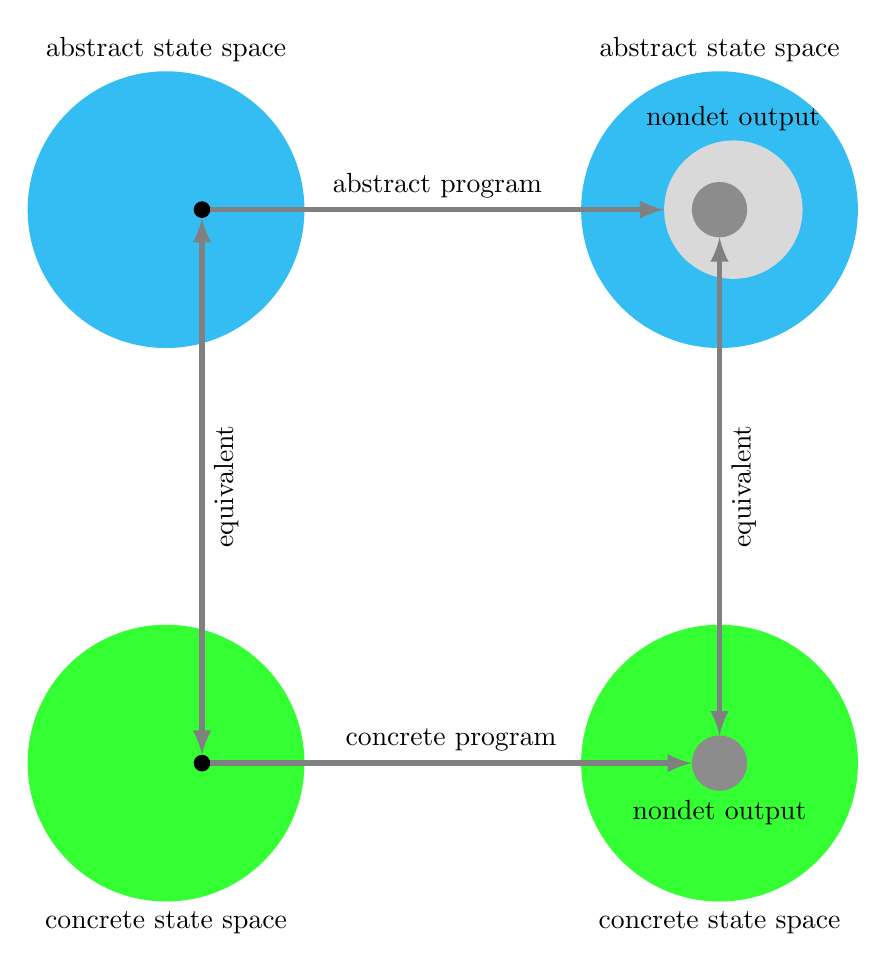
\begin{tikzpicture}[
    dot/.style = {circle, fill, minimum size=#1,
                  inner sep=0pt, outer sep=0pt},
    dot/.default = 6pt
    ]
            % styles
            \tikzstyle{arrow} = [line width=2pt,->,>=latex,draw=gray]
    
            \node (abss) [dot=100pt, fill=cyan!80,label=abstract state space] {};
            \node (abp) [dot, right=-40pt of abss] {};
            \node (abss2) [dot=100pt, fill=cyan!80,label=abstract state space, right=100pt of abss] {};
            \node (abpout) [dot=50pt, fill=gray!30,label=nondet output, right=-70pt of abss2] {};
            
            \node (copout2) at (abpout) [dot=20pt, fill=gray!90, right=-60pt of abss2] {};
            
            \node (coss) [dot=100pt, fill=green!80,label=below:concrete state space, below=100pt of abss] {};
            \node (cop) [dot, right=-40pt of coss] {};
            \node (coss2) [dot=100pt, fill=green!80,label=below:concrete state space, right=100pt of coss] {};
            \node (copout) [dot=20pt, fill=gray!90,label=below:nondet output, right=-60pt of coss2] {};
    
            \draw [arrow] (abp) -- (abpout) node[midway, above] {abstract program};
            \draw [arrow] (cop) -- (copout) node[midway, above] {concrete program};
            \draw [arrow, <->] (copout) -- (copout2) node[midway, right] {\rotatebox{90}{equivalent}};
            \draw [arrow, <->] (abp) -- (cop) node[midway, right] {\rotatebox{90}{equivalent}};
    \end{tikzpicture}}
\end{figure}
\end{frame}











% \subsection{Approach}
% \begin{frame}
%     \frametitle{Prior work}
%     \begin{itemize}
%         \item Follow along with seL4's methodology for proofs
%         \item Use seL4's existing tools
%         \item Use existing specifications (network stack has been built before)
%     \end{itemize}
% \end{frame}


% \subsection{Background}

% \section{Methods}
% \subsection{seL4}
\begin{frame}
    \frametitle{What do we need to write functional code using seL4?}
    \begin{itemize}
        \item seL4 is hard to work with
            \begin{itemize}
                \item use sDDF
                \item use microkit
            \end{itemize}
        \item PDs
        \item memory regions
    \end{itemize}
\end{frame}




\begin{frame}{System software is hard to verify}
    System software is in charge of low-level operations.
    \begin{itemize}
        \item needs to be fast
        \item directly deals with memory and other hardware resources
    \end{itemize}
    These make verification tricky.
    So tricky, people thought it was impossible for a long time.
    \begin{itemize}
        \item until about 2009, most verification dealt with high-level abstract data structures and algorithms
        \begin{itemize}
            \item stacks, heaps, trees
            \item easily formalizable
            \item have to simply assume without proof that basic structures work as intended
        \end{itemize}
        \item in 2009, seL4 proved things from the ground up, only assuming hardware works correctly.
        \item but seL4 doesn't do anything on its own---it's a \textit{microkernel}.
    \end{itemize}
\end{frame}








% \subsection{Formalizing program execution}
% \subsection{What does it mean to verify a program?}

% \section{Results}
% \subsection{Current state of proofs}

% \section{Discussion}
% \subsection{Remarks/Conclusion}
% \subsection{Pure function vs pure state transformation vs hybrid}
% \subsection{Prior work}





    
\end{document}


